
% Chapter Template
\setstretch{1}
\chapter{Hardware Deployment in Limited Local Space}\thispagestyle{empty} % Main chapter title

\label{Chapter4} 

\lhead{Chapter 4. \emph{Hardware Deployment in Limited Local Space}}
\setstretch{2}
\begin{figure}[!ht]
 \centering
  
\includegraphics[width=\textwidth]{psXXYborgVan3}
  \caption{Hannah Epstein\\ psXXYborg at VideoFag, 1995}
\end{figure}

\begin{figure}[!ht]
 \centering
  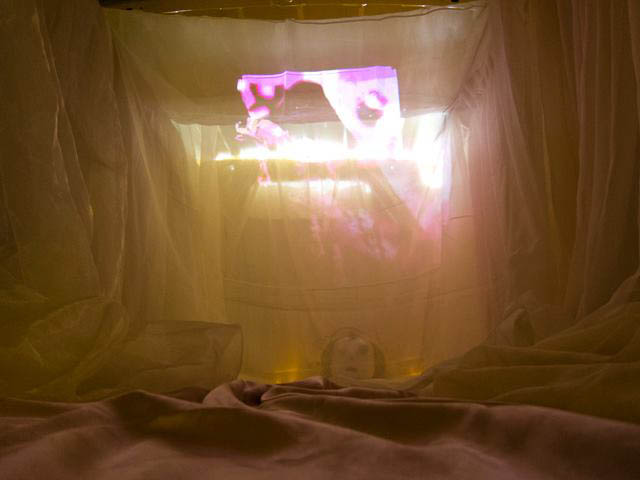
\includegraphics[width=\textwidth]{psXXYborgInterior}
  \caption{Hannah Epstein, Alex Leitch, Sagan Yee\\ psXXYborg at VideoFag, 1995}
\end{figure}
\newpage
\newpage

\section{Public Installations}
During the course of this project, games made with ScreenPerfect had many public outings. We installed psXXYborg specifically in a variety of spaces, and there were a number of design approaches to the construction of those spaces, governed mainly by Hannah Epstein.

\newpage

\begin{figure}[!ht]
 \centering
  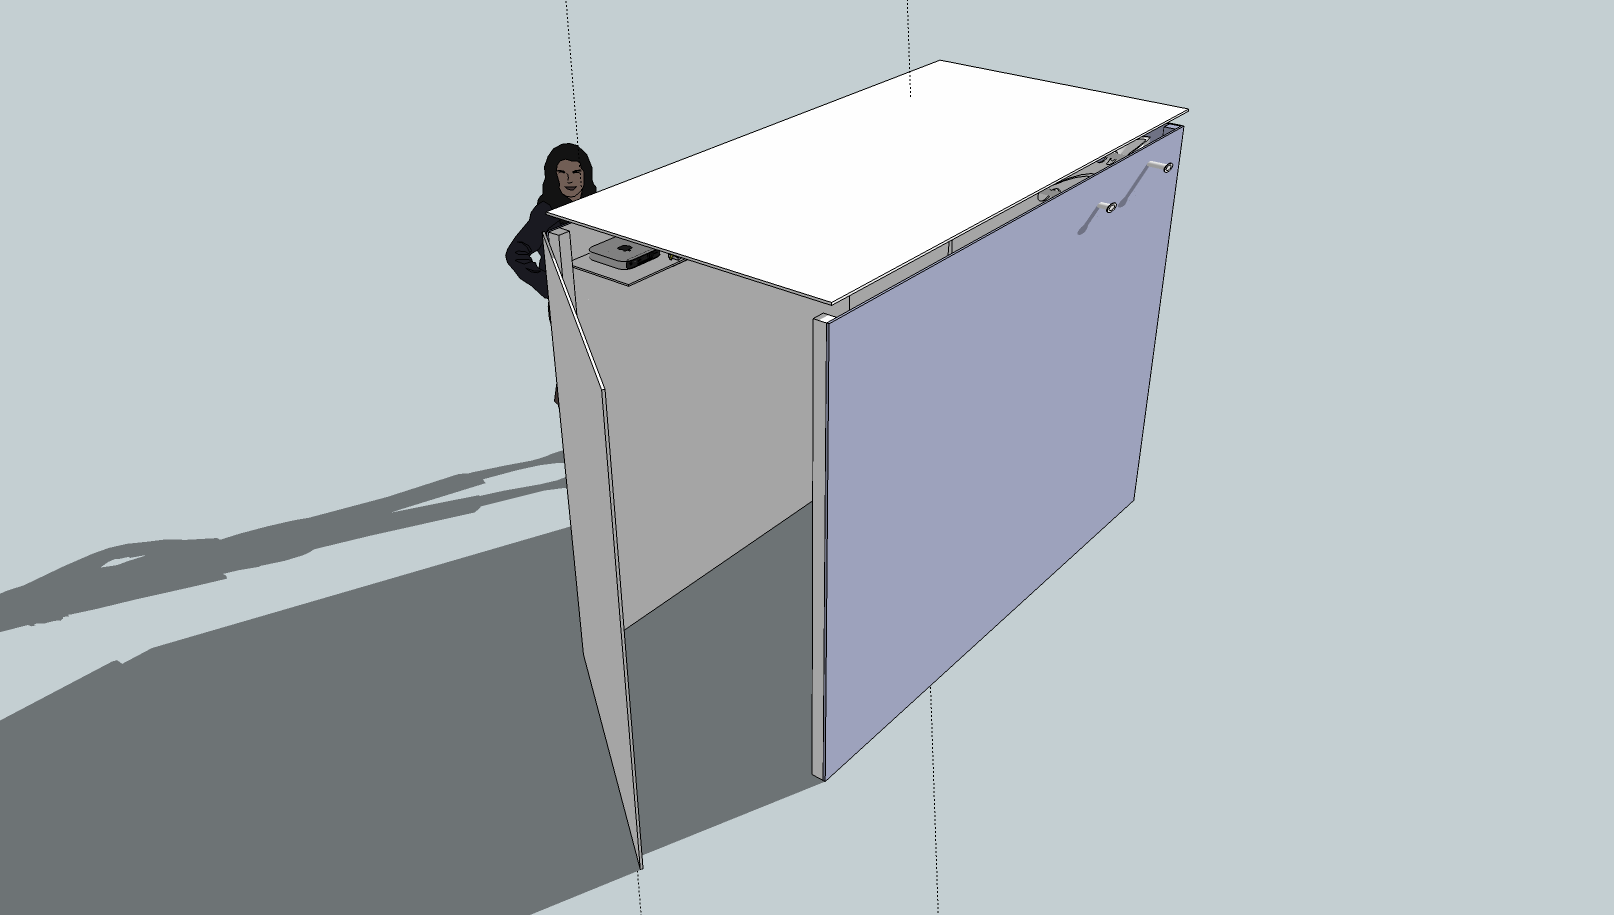
\includegraphics[width=\textwidth]{psXXYborgBox}
  \caption{Alex Leitch\\Concept for collapsible projection space 2013}
\end{figure}

\begin{figure}[!ht]
 \centering
  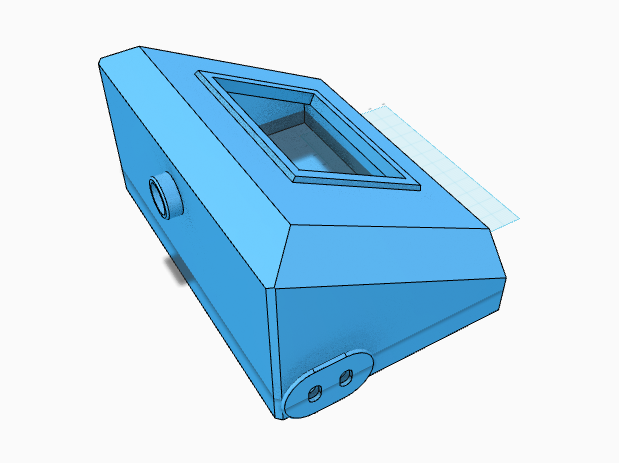
\includegraphics[width=\textwidth]{projectionBox}
  \caption{Alex Leitch\\Concept for portable arcade box, 2013}
\end{figure}

\newpage

\section{Hardware Design}
There were many hardware difficulties associated with early builds of screenPerfect as psXXYborg. The software is dependent on open wiFi and high bandwidth, a stable computing system, a variety of tablets and other devices, and none of these things are confirmed to work together. Idealistically, the software is open. In reality, it is incredibly difficult to build a new software system to work on broad platforms, and this ended up being an unrealistic goal.

After installing PornGame at the Art Gallery of Ontario for a Long Winter event, even the software developed by Miso failed repeatedly to load correctly on a variety of devices. This resulted in the need to reprogram the psXXYborg build of the software to work within a limited network, and from there, I began to research what it would take to adequately display these time-based works. The answer seemed clear: A limited hardware system with a consistent environment, similar to a video game console such as the Super Nintendo Entertainment System. 

With that in mind, I acquired a Raspberry Pi, a new type of microcomputer designed to be used for learning and prototyping new systems. The chief problems on display by screenPerfect were connecting at all, running the application consistently in hot temperatures or unreliable environments, and getting the various videos to display adequately on mobile and non-mobile systems. In addition, the many installations of various games in public began to imply that people love interacting with things, but that computers are unreliable in a public environment. 

I observed that people are willing to use their smartphones publicly, but mainly to access the external internet, or messaging services while they are in public. ScreenPerfect, which relies on the form factor of a mobile device as well as a powerful multipurpose computer, did not seem to work so well in this context.

This led me to consider how people interact with the internet publicly, and to consider topics of privacy and public space, and how these problems have already been solved by galleries and coffee shops wishing to offer their clientele data services to promote engagement.

In public spaces, internet is supplied by wiFi, which comes through a specific type of router known as a "captive portal." A user will walk into a shop, attach to a network, and "sign" an agreement to make use of the wiFi within that space. 

Normally, the wiFi will then give them access to the external internet - the internet as supplied by a major ISP. This is not necessarily what needs to be supplied, however. In the Subnod.es project, hosted by Eyebeam in NYC, users pair to a captive portal which is also a server, supplying access to an entirely private chat room, which is available only to users on the network supplied by the captive portal itself. 

This seemed like an excellent answer to the question of how to supply screenPerfect applications so that users can pair to them in an intuitive way, with a minimal amount of hardware that is easily maintainable, and I therefore set about building a Raspberry Pi that would supply two things: a wiFi signal and a server that serves an instance of screenPerfect where users can experience at least one, but hopefully more, screenPerfect games. 

In this, I hoped to address a few problems. The first is that downloading applications to a smartphone seems invasive, particularly if those applications are experimental or site-specific, as - post-psXXYborg - I think that screenPerfect games are when they are at their best. The next is that web applications are very much not user specific - they can be experienced anywhere while they are on the open web, even if their content is intended to be restricted to a specific type of installation, or requires it for best use. 

A small, portable piece of resilient hardware (a Raspberry Pi stores its entire operating system on a single SD card) seemed like an excellent answer, which would provide an appliance-like container to serve this software, and also provide a solution to the problem of external bandwidth reliance. By serving the application locally, there is no reliance on an outside pipe. A copy of the game can be sold, customised, and stored in a collection, if such is desired, or installed in any kind of specific cabinet for later use. 

I decided on the Pi specifically because it is a cheap, accessible, reproducible system with a broad community of access and support, with the ability to include hardware controls where necessary. This type of system could also be built out on any leftover PC using a build of the Debian linux system.

\section{Physical Deployment on the Raspberry Pi}
One of the earliest problems screenPerfect has been compromises in how the software is served to players and artists. Reliance on public internet is difficult, because the internet is not always available. WiFi is taken for granted in most institutions, but it is not always reliable, and the most interesting installation zones, such as the forest, may not have internet available at all. 

There are other challenges to public deployment, such as leaving a valuable production environment out in public, or requiring a technician to look in on specialized equipment. Both of these restrict the venues permitted for public display of work. Also limiting are instances where work should be deployed near people consuming alcohol, which is notoriously bad for electronics.

This chapter addresses my central idea on how to repair the gap between excellent idea for web-based deployment, and the physical reality of gallery spaces with sharply limited resources available for persistent software deployment. 


\newpage
\begin{figure}[h!]
 \centering
  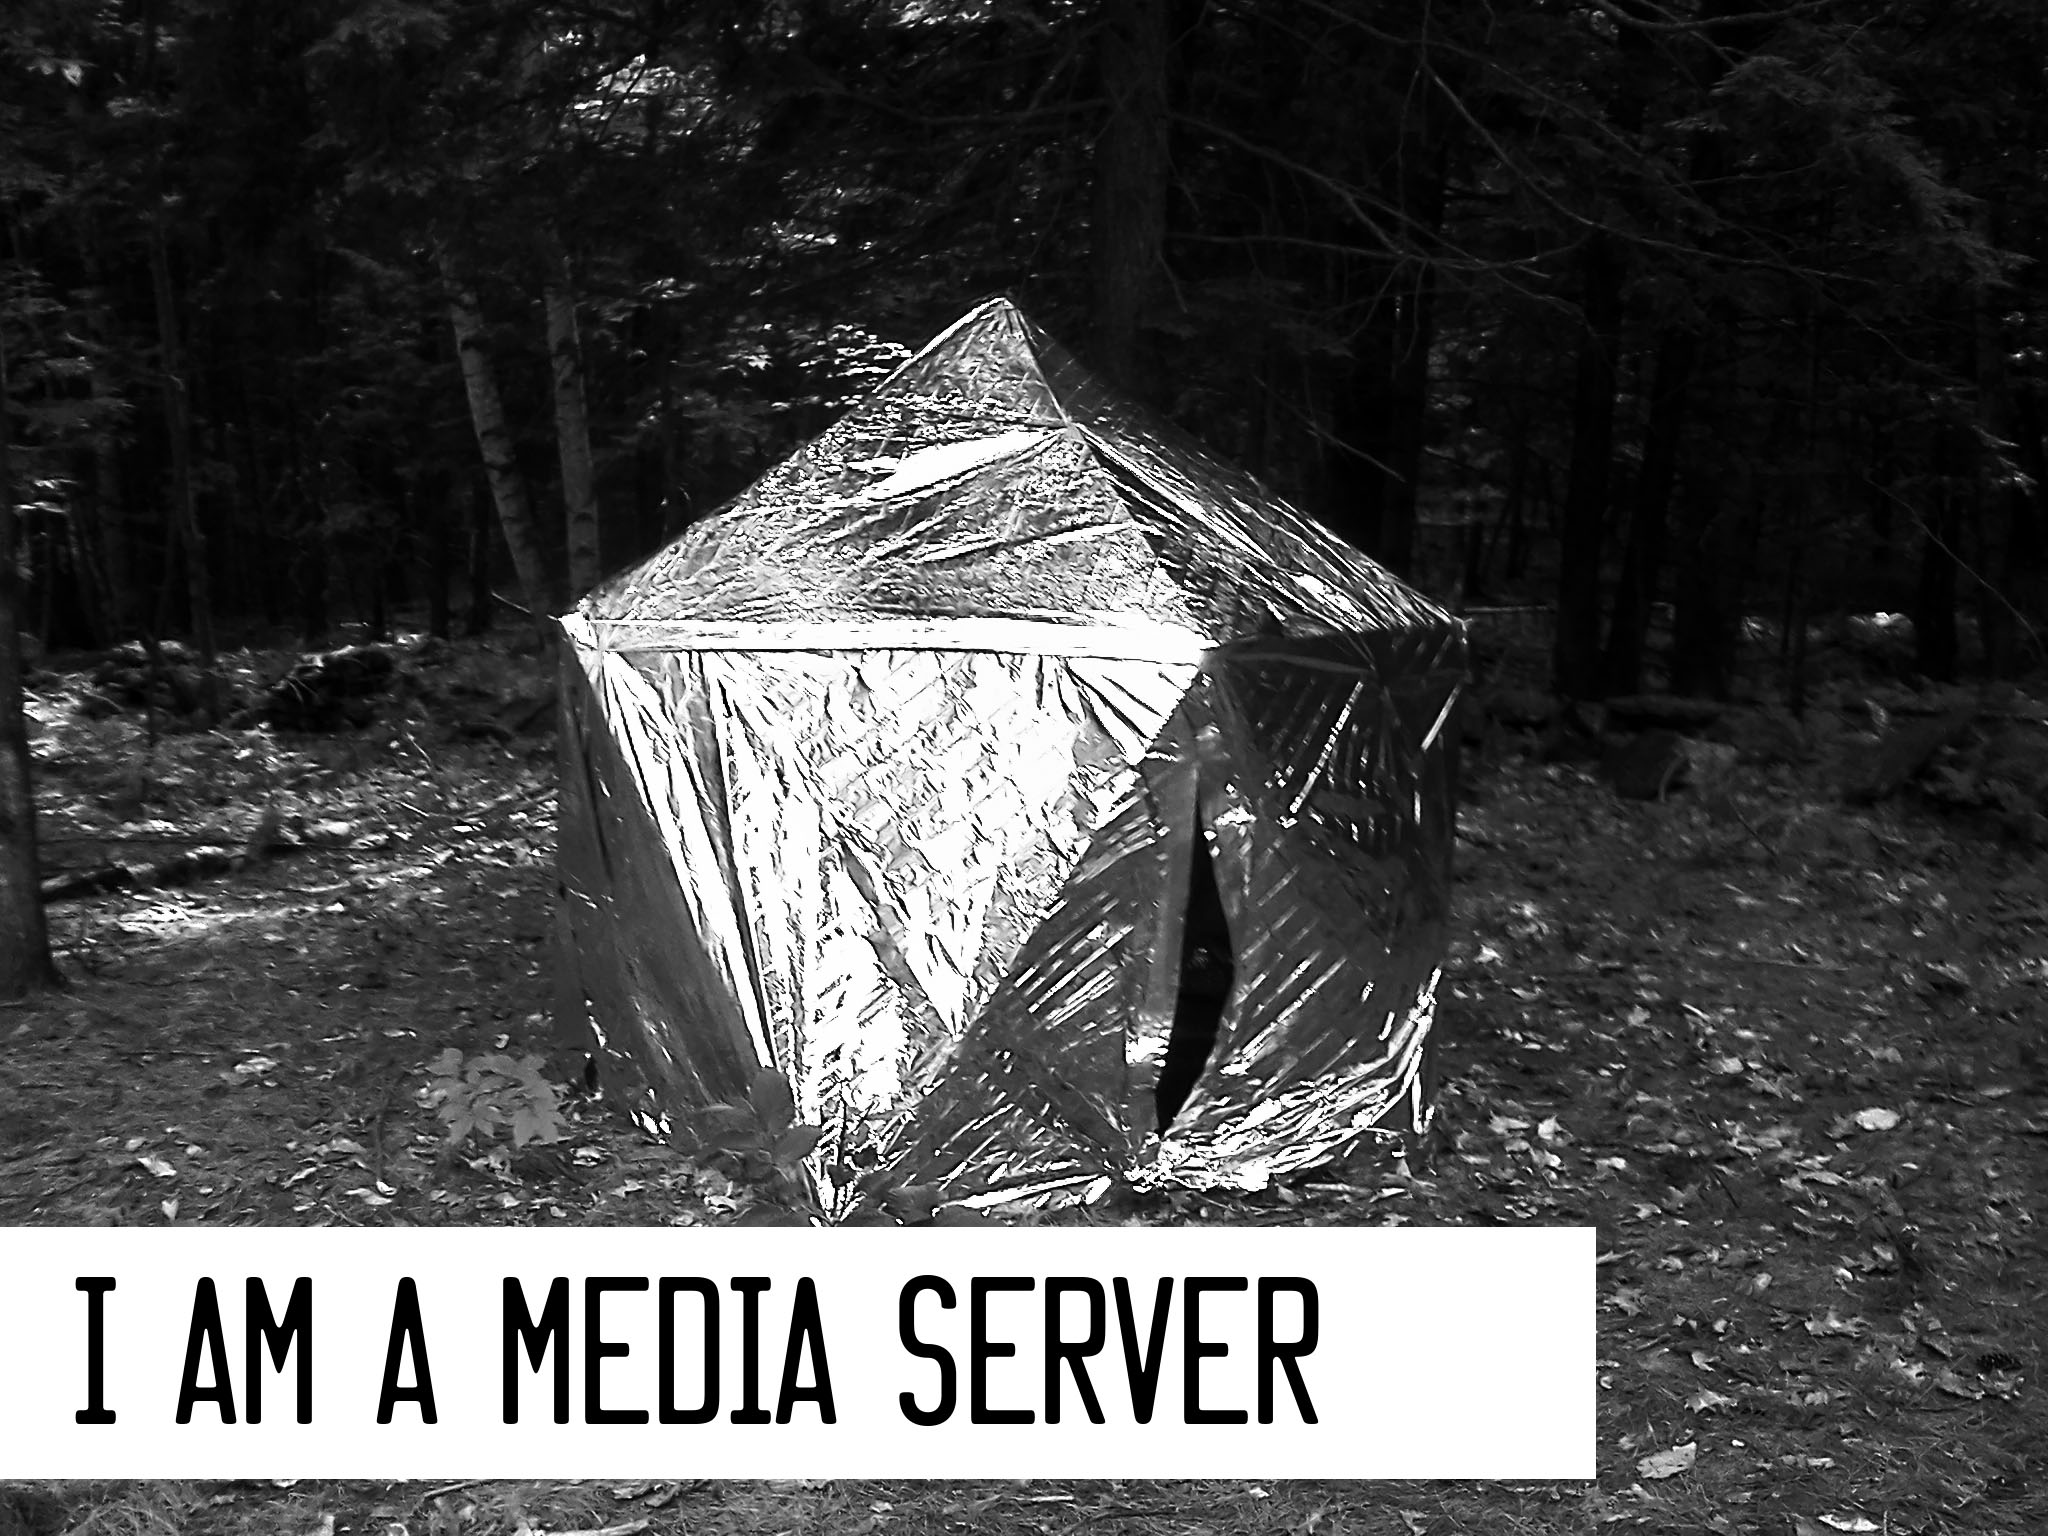
\includegraphics[width=\textwidth]{Seizuredome2}
  \caption{Abe Shulz and Sage Kochavi\\Seizuredome at FireFly 2013}
\end{figure}
\newpage

\subsection{Problems and Complications in Display}
These issues have been revealed through various installations of screenPerfect in public space. Exhibiting in a van, in a park, and in an institution with limited bandwidth revealed a clear set of questions around improving installation circumstances. screenPerfect needed to be an arcade box, similar to those used for years in fighting games in bars.
 
Some brainstorming resulted in the following scenarios that a reasonable arcade machine would need to address in order to present advanced work to the new, highly exclusive exhibit scenarios. 

\begin{enumerate}
\item Data service to an external source cannot be assumed to be available. 
\item The exhibit is assumed to be displayed in public
\item The environment is assumed to be meterologically hostile - hot or cold, wet or very dry, and to be hosting at least one party, such as an art opening, possibly with music
\item The exhibition is assumed to be supervised by technically untrained people.
\item The emphasis of the work should be on the work's display, rather than on a laptop screen.
\item The collectors of the work are assumed to have extremely limited resources for ruggedized workstations.
\item Any host-provided data carriage for external connection - wiFi - is assumed to be overloaded by default.
\end{enumerate}

 These are all very real constraints that impact display of new media art. We use computers for work and play, but we still separate our lives into periods when we pursue one or the other, and we still have boundaries between our personal and public lives. To use the same machines to display art as we do to build the work is to reduce the work from something approachable to any other tab in a computer. New media works especially must be seen within their exhibition context to be understood.

\subsection{Subnod.es and Public Private Space}
This project has a precursor using similar technology builtat Eyebeam in New York in 2013. Subnod.es uses a captive portal similar to my own, based on the inexpensive Raspberry Pi framework, to display a chat client to only the local environment. The differences are substantial, although mainly located within the code. Subnod.es relies on an external DNS being made available via the actual subnod.es software, and depends on a different collection of software to serve the portal proper. It is also built such that those library dependencies are inseparable from the main project script.

The chief concern of subnod.es I have not yet mentioned: subnod.es was built as a response to concerns about communications privacy in North America under the NSA. Specifically, the author is concerned that people behave differently when they are watched, a subset of the concerns generally associated with panoptica and totalitarianism. While I have not specifically structured screenPerfect's Art Portal to address these concerns, it has been built to be largely private. It serves an application to a limited selection of a public space.

The assumption of the Captive Portal Art Machine is that galleries have limited resources, but that people who go to art galleries almost certainly have access to a smart phone, which is a form of private space. Smart phones are people's own homes, and are built to assume that they will stay with their owners at all times. This means that to install an app is to ask a lot of a viewer: specifically, it is to ask someone to bring an application into their private space without getting to sample it first. To contrast, serving that same application on the broad internet is to entirely delimit the context the art may be experienced within, which reduces its scarcity value to almost nothing while simultaneously removing the curator's ability to set the context of an exhibition experience. This means that it's unlikely an artist can be compensated in any conventional sense, despite their large audience, and also means that the curation of the exhibit is no different than the "curation" found on Tumblr. This seems to me to be a negative outcome.

A better outcome might be to make a limited public space available in a private context, and this is what we are doing when we ask that people open their phones and look at a website. The Internet is, famously, the new public space. By presenting a web application using public technology within the exclusive context of the gallery - or desert, or forest - we take control again over how our art is presented, and from there, how it can be consumed. A gallery or exhibit space can be set up very specifically for the benefit of an audience in a way that the internet in general cannot be, and web technologies are uniform and affordable in the way that more custom projection design software is not.

This sense of limited private space is key to the code-switching that human communication relies on. We are not the same people in public as we are in private, and we are again different people when we are in different publics, work to the street to school to the gallery. Technology that sensitively addresses these different code contexts seems likely to benefit its authors and its users both.
 
 \subsection{Materials and Supplies}
\textbf{Raspberry Pi}
The Raspberry Pi is a full linux computer the size of a large credit card. A Raspi runs Debian linux off of a common SD card.
\textbf{32Gb SD Card for Raspberry Pi}
This is where we place the operating system and software for the Pi.
\textbf{USB wiFi dongle}
Edimax-based wiFi USB dongle, for serving wiFi hotspot on the Pi.
\textbf{USB flash memory}
For transferring or storing complete programs authored on external systems.
\textbf{Keyboard and Mouse}
For initial computer setup.
\textbf{Ethernet Cable}
Standard cat5 ethernet cable for programming remote.
\textbf{HDMI TV and cable}
Used as a monitor for the Raspberry Pi.
\textbf{Micro USB and power supply}
Power for the pi.
\textbf{Mac or PC computer with USB ports, ethernet port, SD Card reader}
Required for raspberry pi setup.

\section{Background for Linux Commands}
sudo means "do this now even if I appear to have insufficient user permissions" in Linux 
apt-get is an inherited "package manager" from Debian linux. "Dependencies" are the software your software requires to run, Debian uses apt-get to manage them.
Things that follow sudo are commands.

\section{Setting Up The Raspberry Pi}
\subsection{Windows 7 SD Card setup and first boot}
This section is written for a Windows 7 environment, and is based on the common tutorial at \url{http://learn.adafruit.com/adafruit-raspberry-pi-lesson-1-preparing-and-sd-card}
\begin{enumerate}
\item Connect your main computer to the internet.
\item Download the most recent Raspbian distribution image from \url{http://www.raspberrypi.org/down}
\item Download Win32DiskImager from the greater internet. This is preferable because it allows you to write image backups to your harddrive.
\item Using Win32DiskImager, write your Raspbian distro to your SD card on your main computer.
\item Eject the microSD card and stick it into the Raspberry Pi.
\item Plug in your keyboard, and plug a mouse into your keyboard.
\item Plug in your HDMI cable and monitor. Turn them on.
\item Plug in the MicroUSB cable for power to the Raspberry Pi.
\end{enumerate}


\subsection{Configuring Raspbian}
Once the RasPi is turning on, it needs to be set up to include all of its software. Turn the Pi on, and wait until the blue configuration screen comes up.
Figure 4.3: Early RasPi Configuration Screen

\begin{enumerate}
\item expandrootfs Expand the boot system so that you will not run out of onboard memory for software.
\item memorysplit Reduce the GPU to minimum, because we will be using the raspi as a headless server from the command line.
\item changepass Change the password so that the Raspberry Pi will be less easy to hack.
\item ssh Enable SSH so that the pi will be accessible from an external computer.
\end{enumerate}

When done, select finish to exit.
Type sudo reboot to restart the raspi.

\section{Software Setup for External WiFi Access}
A wiFi antennae can be used for one purpose at a time: it can either be used to access the external internet, for acquiring software to install into the raspi, or it can be used for serving a hotspot. It cannot do both at the same time. To load the pi up requires external access, so we will be loading that first. You must configure your wiFi before plugging in your wiFi antenna. 

In Linux, there is warning you if you mistype a folder name, say, adding an "s" to "network" to make it "networks." If you would like to confirm your folder name is correct, try typing "ls /etc/" to list the contents of that directory. Network is a default folder, and Interfaces is already present at first boot, so you can make sure your things are all there before you really get started. The way to tell you have done something wrong is if you type the below command and an empty new file opens. You are editing a file here, not creating one.
 At your console prompt, type the following:

\begin{lstlisting}
sudo nano /etc/network/interfaces
\end{lstlisting}

This opens a text editor called 'nano.' Enter the following into it.
\begin{lstlisting}
auto lo

iface lo inet loopback
iface eth0 inet dhcp

allow-hotplug wlan0
auto wlan0

iface wlan0 inet dhcp
wpa-ssid "network name, commonly called an ssid, goes here"
wpa-psk "password"
\end{lstlisting}

Then type CTRL-X and Y to save your file.

\begin{lstlisting}
sudo halt
\end{lstlisting}

Plug in your wifi antennae, pull the Raspberry Pi's power cable, and plug it back in. This should make the raspi's antennae turn blue as it turns on. This little blue LED will frequently be the only way to tell something is going correctly or incorrectly, so it is an excellent tell that your machine is running.

Plug in your wifi antennae, pull the Raspberry Pi's power cable, and plug it back in. This should make the raspi's antennae turn blue as it turns on. This little blue LED will frequently be the only way to tell something is going correctly or incorrectly, so it is an excellent tell that your machine is running. 

The case in the following figures is a modification of an open-source design supplied by Thingiverse.com user DrewTM. It is Thing \#114244 and can be found at https://www.thingiverse.com/thing:114244.

\newpage
\begin{figure}[h!]
 \caption{Raspberry Pi with functioning wiFi antenna}
 \centering
  \includegraphics[width=0.5\textwidth]{raspiWiFi}
\end{figure}

\begin{figure}[h!]
 \caption{Raspberry Pi in Thingiverse case}
 \centering
  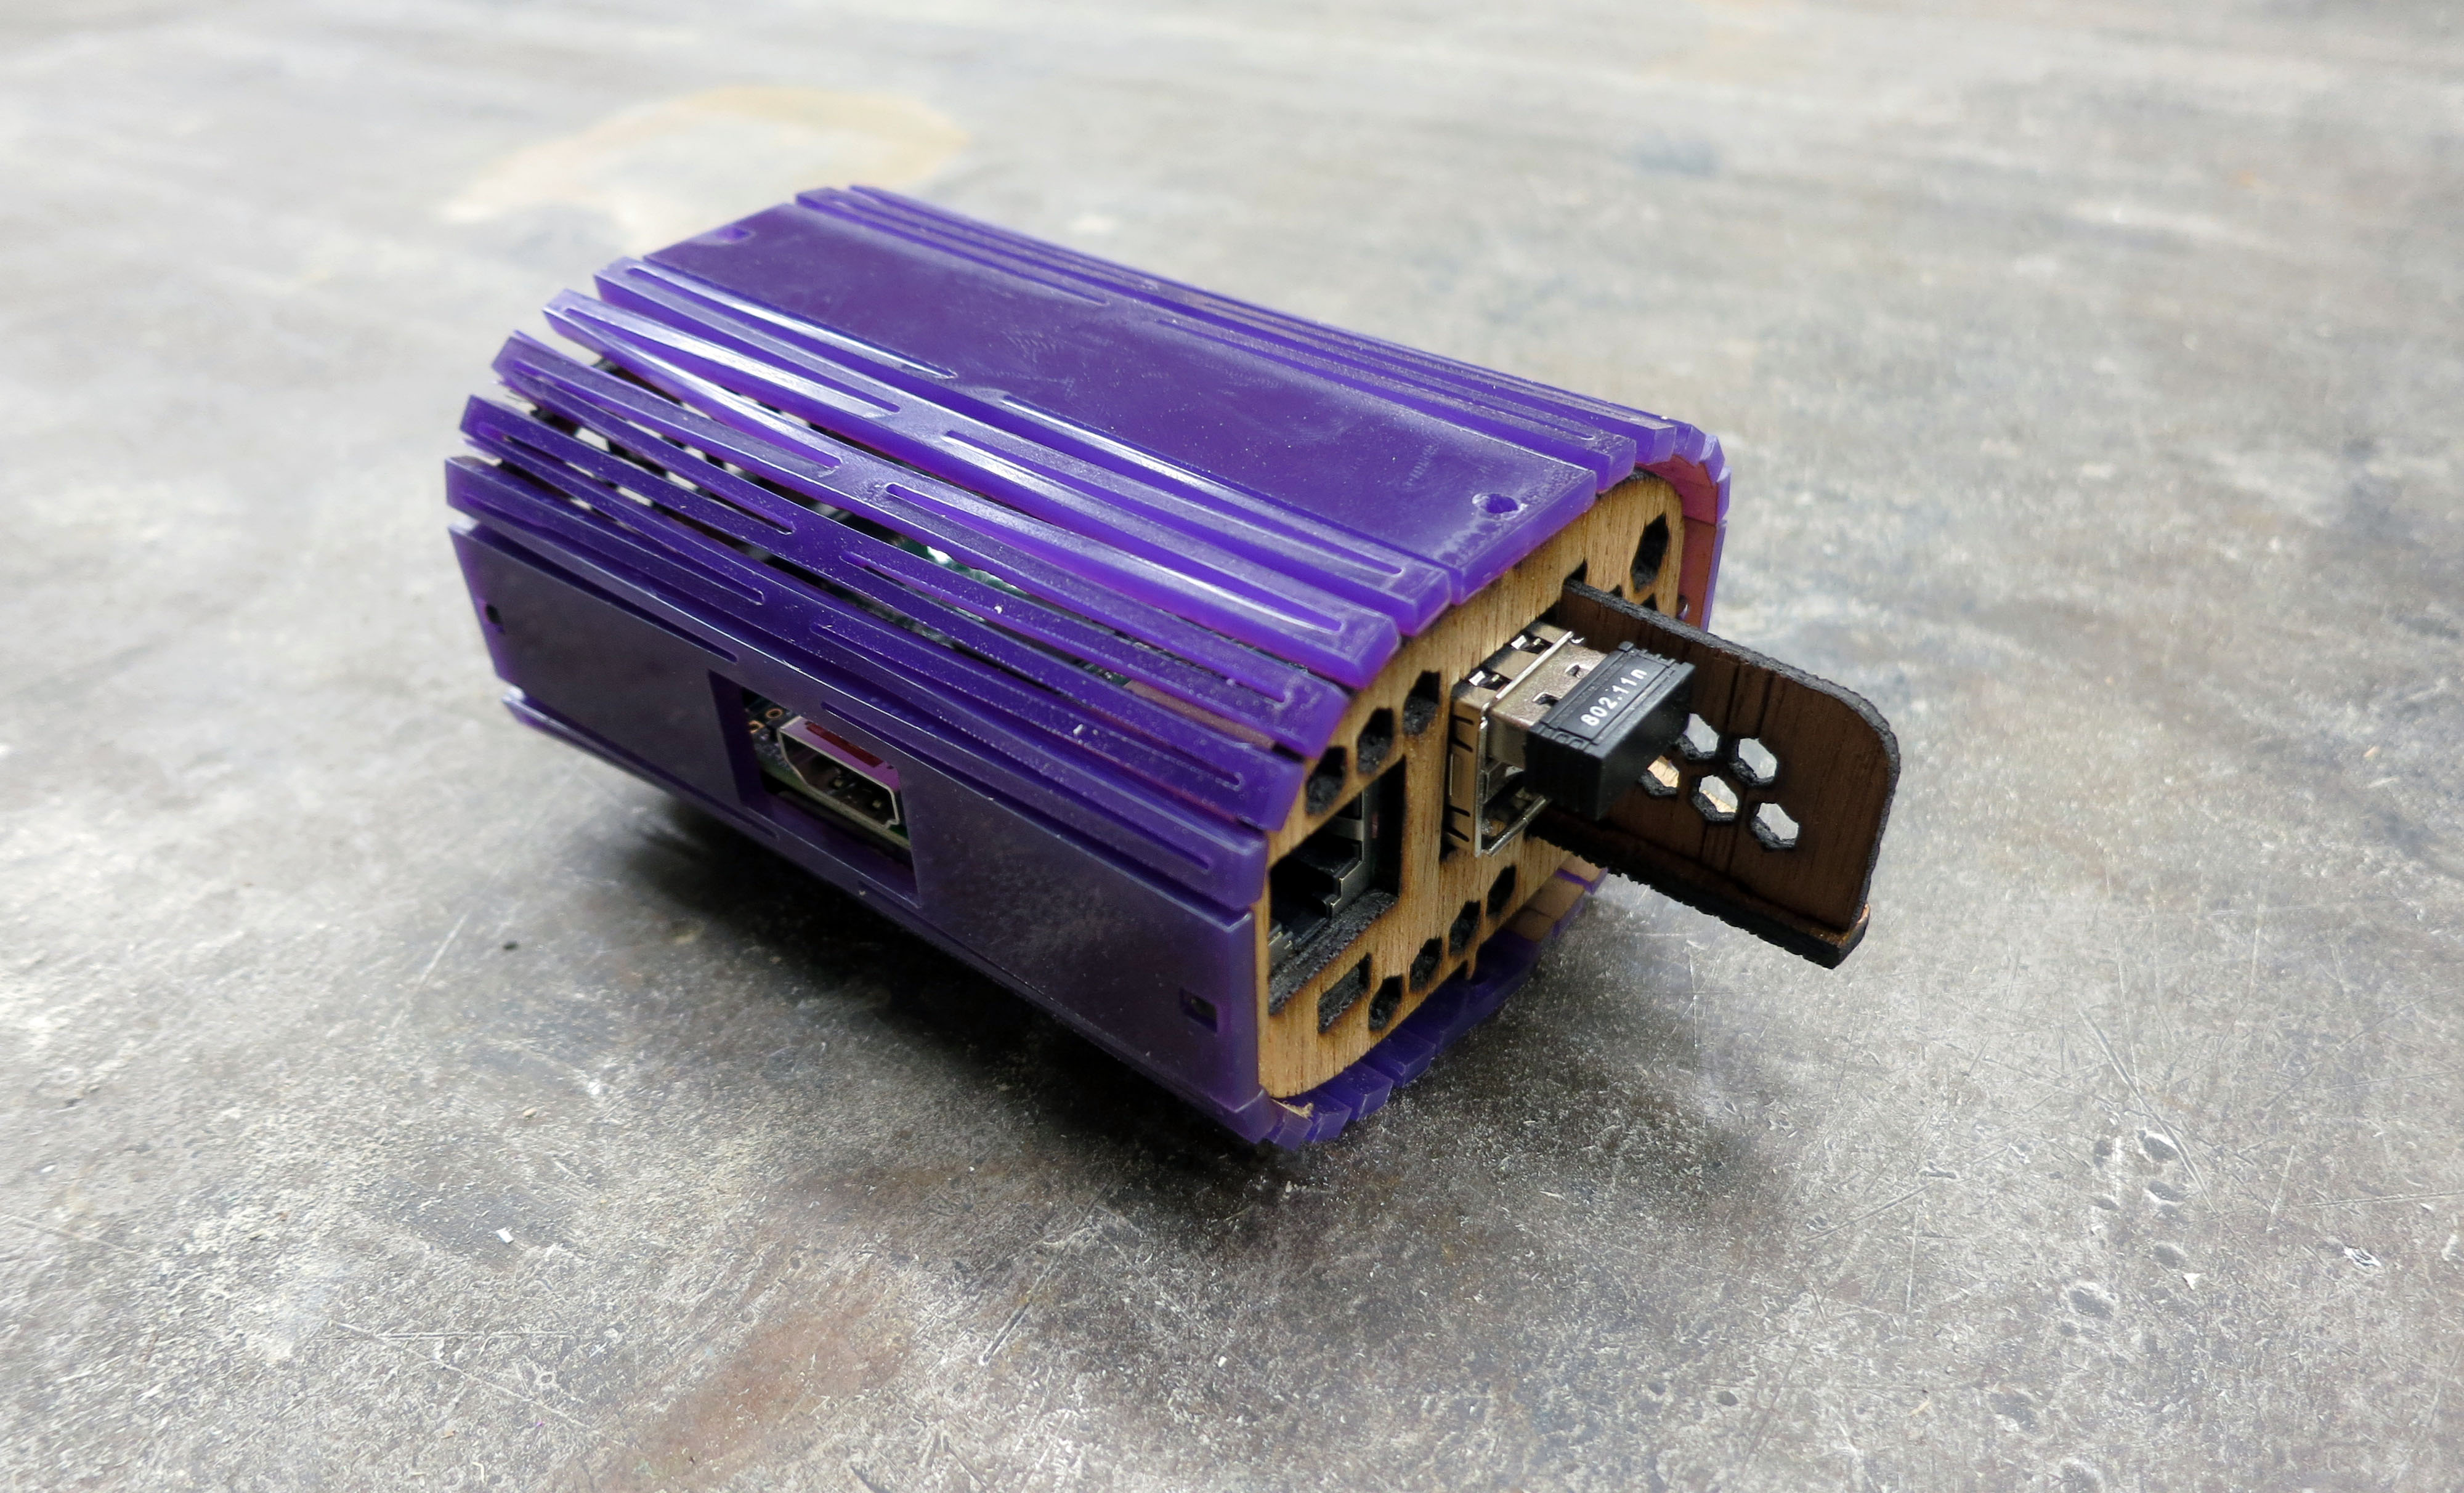
\includegraphics[width=0.5\textwidth]{raspiCase}
\end{figure}

\newpage

If all went well, you've now connected to your own supply of wireless internet. This will not work if you are using an 802.1x network, such as those within OCADu. On your own home network, however, type:

\begin{lstlisting}
sudo apt-get upgrade; sudo apt-get update
\end{lstlisting}

This will upgrade your rasppi to whatever the latest agreed-upon package lists are, then update those packages to their most recent approved version.

\section{Installing Node.JS}
\subsection{Why Node?}
I've chosen to install Node because it is the software framework I selected to run the new game engine built in Part 1 of this thesis. Node is a new framework designed to get Javascript running on a server. There are advantages and disadvantages to this approach. The advantages are that JavaScript is a beautiful, minimal language that is relatively easy to learn. The disadvantages are that there is a heavy public bias against JS due to its years as a client-only language designed to manipulate what are known as Document Object Model (DOM) elements in-browser.

The brilliance of Node is that it replaces the need for a specific input-output window, replacing that definition requirement with any internet browser. Node, backed by Google's V8 engine, currently works best on Chrome, but it can interact with any browser.

Node is therefore easy to use, and easy to program for from the perspective of a mainly web based development chain. 

\subsection{Installation Instructions for Node.JS}
Create a directory for Node to live in by typing the following at prompt.
\begin{lstlisting}
sudo mkdir /opt/node
\end{lstlisting}

Acquire the node "tarball" - compressed framework files - via the internet.

\begin{lstlisting}
wget http://nodejs.org/dist/v0.10.2/node-v0.10.2-linux-arm-pi.tar.gz
\end{lstlisting}

Unzip (desticky from tarball) it:
\begin{lstlisting}
tar xvzf node-v0.10.2-linux-arm-pi.tar.gz
\end{lstlisting}

Copy the contents of the newly unzipped folder and paste them to your new directory. This leaves a copy of the tar and a copy of the unzipped tar at their original locations. You can probably remove them using sudo rm when you're sure everything is where it should be.

\begin{lstlisting}
sudo cp -r node-v0.10.2-linux-arm-pi/* /opt/node
\end{lstlisting}

Edit - or create - a .bash_profile file, which is a type of script that runs when you turn on the pi. In this case, it runs and tells Node that it exists on your computer, so that typing node runthisprogram will do something. What is a .bash_profile?

From your root directory, to open a new nano text file:
\begin{lstlisting}
sudo nano .bash_profile 
\end{lstlisting}

Then add the following and save it to your new .bash_profile file...

\begin{lstlisting}
PATH=$PATH:/opt/node/bin 
export PATH
\end{lstlisting}

Control-X, Y to save it.

Node lives in the \texttt{/opt/node} directory you created above. This adds the commands "node" and "npm" to what are called "environment variables." If you are curious, and god knows you must be to play with a raspi, you can type \texttt{ls /opt/node/bin} and see the little programs sitting there in their bin.

\section{Testing Node}
Node will need to be able to fetch its own packages separately from the raspi from the internet in order to run some of the monitoring software I've chosen to use. Particularly, you will need the \texttt{forever} package.

\subsection{Selecting Monitoring Software}
\texttt{forever} has ultimately been the software I've decided on to monitor and run screenPerfect, because it is a node-native package that keeps things running even when they crash. There are other software packages used for broader deployment, such as Monit, which installs to your Debian parcel rather than to Node. Monit typically runs with what is called an HTTP Proxy, which can be written directly in Node or installed independently. In a full deployment build, Monit and HAProxy would be preferable to Node alone, because this follows the best practice of separating out different programming elements from one another in production. Monit and HAProxy can also deploy applications above and beyond Node itself, which is preferable for things written in Python, for example. 

For this example, though, \texttt{forever} works well. It provides monitoring to tell us what the application is doing, and automatically restarts node applications when they crash. Were I deploying this such that it could keep an eye on the internet, which I am not, I would also include \texttt{nodemon}, as is recommended by the Subnod.es project. \texttt{nodemon} monitors your development code and pushes changes from a central server to your deployment automatically.

That is outside the scope of this paper at present. 

\subsection{Installation of Node Modules}
To install a node package - or "module" - you type 

\begin{lstlisting}
npm install PACKAGENAME
\end{lstlisting}

To install one globally, type
\begin{lstlisting}
npm install PACKAGENAME -g
\end{lstlisting}


To absolutely force install:
\begin{lstlisting}
sudo su
PATH=/opt/node/bin/:$PATH
npm install PACKAGENAME -g
exit
\end{lstlisting}

To install \texttt{forever} and \texttt{nodemon}
\begin{lstlisting}
npm install forever -g
npm install nodemon -g
\end{lstlisting}

To run \texttt{forever} and \texttt{nodemon} together....
\begin{lstlisting}
forever start /usr/local/bin/nodemon /path/to/YOURAPP.js
\end{lstlisting}

\subsection{Troubleshooting NPM installations}
When I tried to install \texttt{forever} the first five times, it timed out, gave me a 404 error repeatedly, and declared I had insufficient permissions to do a global install. This is where computer science faith, confidence, and patience come in. When the install did not work for half an hour, I took a break, came back, and discovered that it installed the next day.

This process is heavily dependent on a massive network of computers and other people. In development, it is quite likely things beyond one's own control are going to go wrong. Going for a break will help you keep patient.

\section{SSH via Direct Ethernet Connection\\ and WiFi Internet Access}
Eventually, you will need both of the powered USB slots on the raspi for a USB key and for your wiFi. In addition, the raspi doesn't have the power to drive a monitor and consistently serve wiFi out of its USB ports. To get around this, it is most convenient to be able to SSH in to your device. Although it appears to be best practice to use the wpa_supplicant file to store how you wish the Raspberry Pi to connect to the internet, I have had limited success with it, likely because I am not configuring a static IP for my raspi properly.

My \texttt{/etc/network/interfaces} file looks like this:
\begin{lstlisting}
auto lo
iface lo inet loopback

auto eth0
iface eth0 inet static
address [MY MAIN TERMINAL'S ETHERNET IP PLUS ONE]

auto wlan0
allow-hotplug wlan0
iface wlan0 inet dhcp
   wpa-ssid "network name here"
   wpa-psk "dubiously secure password"
\end{lstlisting}
 

\begin{lstlisting}
sudo nano /etc/default/ifplugd

### MANY TALK, HOW COMMENT, SUCH WARNING ###
INTERFACES="eth0"
HOTPLUG_INTERFACES="eth0"
ARGS="-q -f -u0 -d10 -w -I"

SUSPEND_ACTION="stop"
\end{lstlisting}

This is an edit of the existing bits, and I can't tell if it will break everything long-term.
Here is what your startup script should read. This ensures that your wiFi antenna turns on, which is likely not something it was doing when you plugged in your ethernet directly.

\begin{lstlisting}
sudo nano /etc/rc.local
#!/bin/sh -e

# Print the IP address
_IP=$(hostname -I) || true
if [ "$_IP" ]; then
 printf "My IP address is %s\n" "$_IP"
fi

# Disable the ifplugd eth0
sudo ifplugd eth0 --kill
sudo ifup wlan0

exit 0
\end{lstlisting}

CTRL-X and Y to save, then \texttt{sudo reboot} open a terminal on your main laptop. On your laptop, at the prompt, enter:
\begin{lstlisting}
ssh pi@[the static ip address you entered under eth0 static above]
\end{lstlisting}

Your \texttt{pi@[static ip]} should appear in your terminal window, which means you can now talk to raspi.
Per usual, to ensure your wifi is still working properly, try a \texttt{sudo apt-get update} or \texttt{ping google.com}, both should return you data.

\section{Backing Up the Raspberry Pi}

Now that everything has been configured for the first steps, type \texttt{sudo halt}, and when the Raspberry Pi turns off, remove the SD card from it. Place the SD card back in your main computer and reboot Win32DiskImager.

Create a new file folder somewhere within your Documents folder. I called mine Raspberry Pi Backups.

In the Write From section of the application, select your SD card, which is probably called boot. In the Write To section, select your new folder. 

Write a copy of the kernel image from the boot card to the new backup directory. Then safely eject your SD Card and re-insert it in the RasPi. It is best practice to form these occasional backups as you proceed through set up. Many of these steps can cause the Raspberry Pi distro to break badly. A backup will save a great deal of time when the inevitable happens.

\section{Mount Your USB Flash Memory Stick To the Raspberry Pi}

\subsection{Configuring Your Mount Drive}
This bears some thinking about, because the \texttt{/media/} folder is for media, and you are instead choosing to run a program off of the drive. Subnod.es suggests making it your \texttt{www} drive, for world wide web. I picked \texttt{/mnt/}.

Find your USB memory by listing the the things plugged into dev:
\begin{lstlisting}
sudo ls /dev/sd*
\end{lstlisting}

If you've been following along, yours is almost certainly named "/dev/sda1".

So make a directory for it to be addressed at:
\begin{lstlisting}
sudo mkdir /mnt/USBSTICKNAME;
\end{lstlisting}

Then mount it to that directory
\begin{lstlisting}
sudo mount -t vfat -o uid=pi,gid=pi /dev/sda1 /mnt/USBSTICKNAME/
sudo reboot
\end{lstlisting}

Rebooting will restart the raspi but also close your SSH session. Watch the lights on the raspi board until they're stable again, about two minutes, then:
\begin{lstlisting}
ssh pi@[static ip]
\end{lstlisting}

Oh look. Your USB drive does not automatically mount at boot. Problem.

\subsection{How to Boot Mount External Memory}

Find out the actual name of your external memory card:
\begin{lstlisting}
ls -l /dev/disk/by-uuid
\end{lstlisting}

Write down the UUID of your USB stick.

This is the most manual way to run this operation, and there is software that handles automatic drive mounting. It is called \texttt{usbmount} and was discarded during this process because it ended up being more convenient to rely on my Node application being loaded directly onto the SD card, rather than from boot.

\begin{lstlisting}
sudo chmod 775 /mnt/USBSTICKNAME
sudo sp /etc/fstab /etc/fstab.bak
sudo nano /etc/fstab
\end{lstlisting}

Add the following to \texttt{/etct/fstab}
\begin{lstlisting}
UUID=YOURUUID /mnt/USBSTICKNAME vfat rw,defaults 0 0
\end{lstlisting}

CTRL-X, Y to save, then
\begin{lstlisting}
sudo reboot
ls /mnt/USBSTICKNAME
\end{lstlisting}

This command should display the contents of your USB key when you go looking for it.

At this point, I have taken a copy of my Node application and moved it to the SD card in a separate directory. Although I have optimistically tried to make this a headless - no keyboard or monitor - box, realistically, lots can go wrong with the SSHing process. You will probably eventually want a keyboard, and it is _much_ easier to store your access point as a single image per card, much like any other video game.

To store your games locally, rather than in the USB stick:
\begin{lstlisting}
sudo cp -r /mnt/USBSTICKNAME /home/pi/YOURDIRECTORYNAME
\end{lstlisting}

\section{Set Up a wiFi Hotspot}
To get started, you will need some more software.

\begin{lstlisting}
sudo apt-get install hostapd dnsmasq
\end{lstlisting}

When everything is done installing, you will be converting your \texttt{/etc/network/interfaces} file to serve a hotspot, rather than connect to the internet. 

Here is what my final \texttt{/etc/network/interfaces} file looks like:

\begin{lstlisting}
auto lo
iface lo inet loopback

auto eth0
iface eth0 inet static
   address 169.254.222.xx #xx is a stand-in for an actual address, not included.

allow hotplug wlan0

## wlan internet connect settings are commented out for easy swap.
#auto wlan0
#iface wlan0 inet dhcp
#   wpa-ssid "network name"
#   wpa-psk "network password"

iface wlan0 inet static
   address 192.168.42.1 #42 is a joke about Douglas Adams, in honour of my thesis advisor.
   netmask 255.255.255.0

\end{lstlisting}

\section{Configuring HostAPD}
\texttt{hostapd} is the software that provides the access point using the Raspberry Pi. It can be tricky, and in order to make it work, it needs to be compiled for one's specific model of wiFi antennae. For the purposes of this paper, we are using an antenna sold and supported by Adafruit. The appropriate compile of the hostapd software is included in the supplementary files to this paper, but can also be found at \url{http://www.adafruit.com/downloads/adafruit_hostapd.zip}.

To install a valid copy of hostapd:
\begin{lstlisting}
wget http://www.adafruit.com/downloads/adafruit_hostapd.zip 
unzip adafruit_hostapd.zip 
sudo mv /usr/sbin/hostapd /usr/sbin/hostapd.ORIG 
sudo mv hostapd /usr/sbin
sudo chmod 755 /usr/sbin/hostapd
\end{lstlisting}
 
Now set up a daemon - a piece of automatic system software - to run the hostapd configuration file on boot.
\begin{lstlisting}
sudo nano /etc/default/hostapd
\end{lstlisting}
Uncomment (remove the hash mark in front of) \texttt{\#DAEMON_CONF=""} and replace that line with \texttt{DAEMON_CONF="/etc/hostapd/hostapd.conf}.
Then type CTRL-X and Y to save your file.

My hostapd file is listed below.

\begin{lstlisting}
sudo nano /etc/hostapd/hostapd.conf

interface=wlan0
driver=rtl871xdrv
ssid=piebox
hw_mode=g
channel=6
macaddr_acl=0
auth_algs=1
ignore_broadcast_ssid=0
wpa=2
wpa_passphrase=berrybox
wpa_key_mgmt=WPA-PSK
wpa_pairwise=TKIP
rsn_pairwise=CCMP

\end{lstlisting}

\section{Configuring DNS access via \texttt{dnsmasq}}

Configuring \texttt{dnsmasq} is straightforward. The installation package comes with an extensive config file, which lives at \texttt{/etc/dnsmasq.conf}, and includes all of the options necessary to turn on a DNS routing service.

To configure your dnsmasq installation, enter \texttt{sudo nano /etc/dnsmasq.conf} and then add the following lines to the top of the configuration file. The configuration file contains all these values commented out already, and may be worth a separate read.

\begin{lstlisting}
interface=wlan0
dhcp-range=192.168.42.2, 192.168.42.50,255.255.255.0,12h
address=/#/192.168.42.1 #redirect all DNS requests to 192.168.42.1
server=/screenperfect/192.168.42.1#3003
address=/apple.com/0.0.0.0
\end{lstlisting}

What the above does is tell the raspi to listen on the wlan0 interface, to the dhcp range between 192.168.42.2 and 42.50, for twelve hours per time a client connects to the wiFi point.  In addition, the portal is supposed to redirect all DNS requests - things like "google.com" - to the Pi's main address, which is - as we can see in/etc/network/interfaces - 192.168.42.1, and from there to the port 3003, on which my particular Node application listens.

In addition, the portal serves a spoof address to apple.com, which helps us to pop up the appropriate page on the captive portal when it is turned on. 

To date, this portion has not proven totally effective. Getting a page to pop up on a captive portal requires a series of correct internet handshakes per device, so it has so far been easier to set the URL by hand on client devices to the Raspi.
 

